\documentclass[12pt]{article}

\title{Hopper: Reinforcement Learning-Based Control on a Wheeled Bipedal Robot \\\large Project Proposal \\ Category: Theory and Reinforcement Learning}
\author{Parthiv Krishna (\texttt{parthiv}) and Aaron Schultz (\texttt{azs})}
\date{CS 229 Spring 2021}

\usepackage{hyperref}

\urlstyle{same}

\begin{document}
\include{graphicx}
\hyphenpenalty=10000

\graphicspath{ {.} }

\maketitle

% Instructions below
\iffalse
Your proposal should be a PDF document, giving the title of the project, the project category, the full names of all of your team members, the SUNet ID of your team members, and a 300-500 word description of what you plan to do.
Your project proposal should include the following information:

    Motivation: What problem are you tackling? Is this an application or a theoretical result?
    Method: What machine learning techniques are you planning to apply or improve upon?
    Intended experiments: What experiments are you planning to run? How do you plan to evaluate your machine learning algorithm?

Presenting pointers to one relevant dataset and one example of prior research on the topic are a valuable (optional) addition. 
\fi
% Instructions above

\section{Motivation}
The problem that we intend to tackle is the application of reinforcement learning techniques to control Hopper, a small robot that the Extreme Mobility team within Stanford Student Robotics has been developing over the past several months. A CAD render of Hopper can be seen below.

\begin{center}
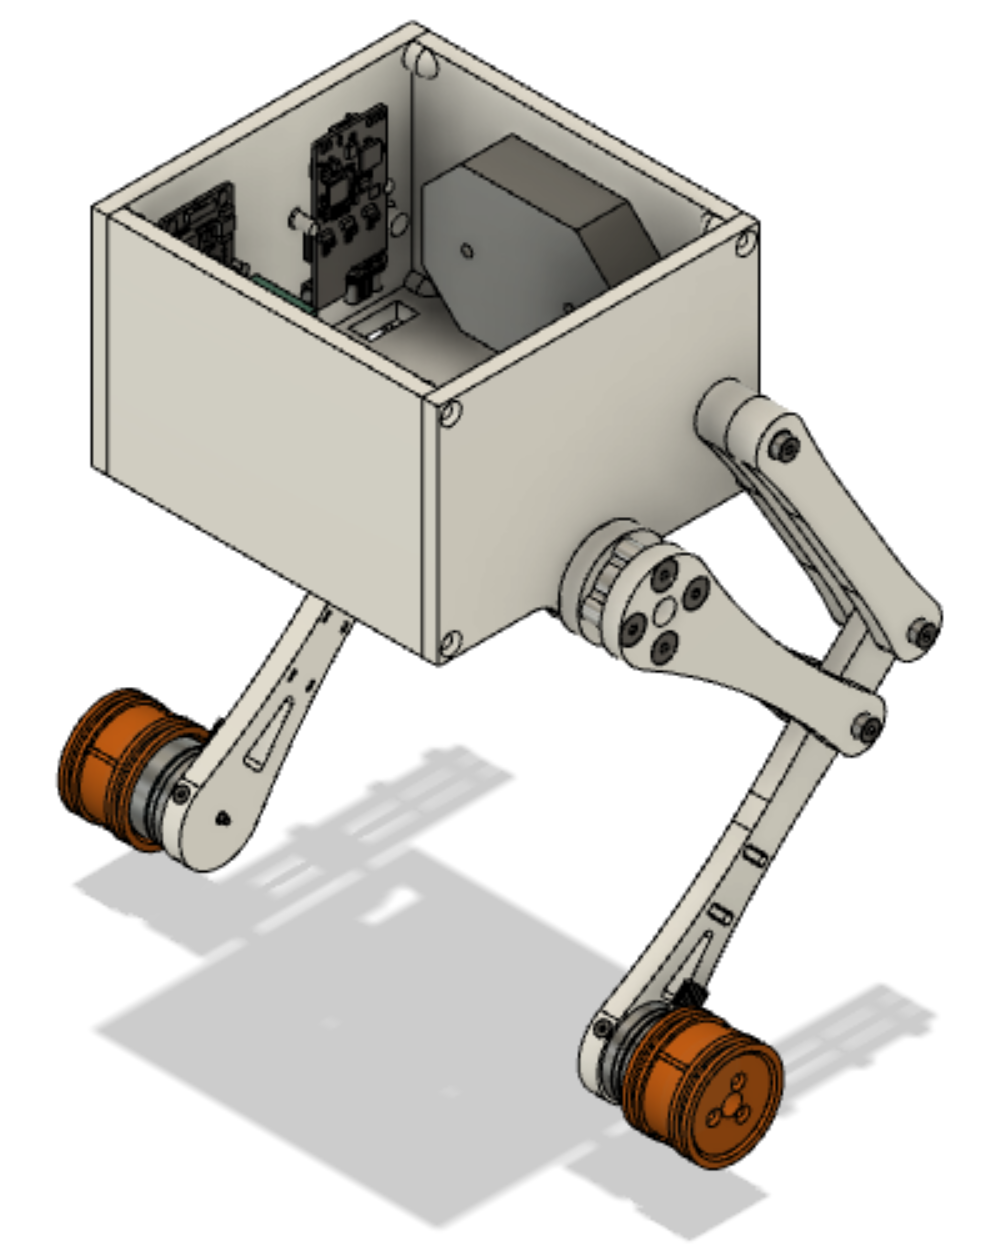
\includegraphics[width=0.3\textwidth]{hopper}
\end{center}

Hopper is a wheeled bipedal robot; in other words, it moves by making use of driven wheels that are attached to the end of two actuated legs. To move effectively, Hopper must maintain its balance while also responding to the desired control input to reach a target position or velocity. Additionally, Hopper can theoretically jump by rapidly extending its legs, and land after jumping by controlling the wheels to maintain stability. 

We propose a project involving the application of a reinforcement learning-based control approach to the robot. As we intended for Hopper to be a platform to test and benchmark different control algorithms, we would like to compare the results obtained by reinforcement learning with those from more traditional control methods like PID.

\section{Method}

We will use reinforcement learning techniques during this project. To actually implement the project, we intend to use some form of physics simulator like PyBullet/OpenAI Gym with a simplified, but dynamically near-accurate, model of Hopper. After the completion of this project, we hope to test the algorithm that we develop on a physical robot as soon as we are able to be on campus. One example of prior research is:

Morimoto, J., et al. A Simple Reinforcement Learning Algorithm for Biped Walking. \textit{IEEE International Conference on Robotics and Automation}, 2004. \href{https://doi.org/10.1109/robot.2004.1307522}{\underline{doi:10.1109/robot.2004.1307522}}. 

\section{Intended Experiments}

We plan to test the algorithm in a few different scenarios, which may include:
\begin{enumerate}
    \item Balancing while staying still
    \item Driving at some fixed velocity
    \item Landing from a jump
\end{enumerate}

We will evaluate our machine learning algorithm by comparing it to a traditional method of control like PID. We will compare these different algorithms on the basis of some chosen metrics, which may include:
\begin{enumerate}
    \item Maximum angle of perturbation from which Hopper can return to stable balancing
    \item Maximum height obstacle that Hopper can drive over
    \item RMS error of Hopper's angle from vertical
\end{enumerate}
\end{document}
